\section{KV-Direct 操作原语}
\label{kvdirect:sec:architecture}
\label{kvdirect:sec:kv-operations}

KV-Direct 将远程直接内存访问(Remote Direct Memory Access,RDMA)原语扩展到\textit {远程直接键值访问}原语,如表 \ref {kvdirect:tab:kv-operations} 所述。
客户端将\textit {KV-Direct 操作}发送到键值存储服务器,而可编程网卡处理请求并发送回结果,绕过CPU。
键值存储服务器上的可编程网卡是一个重配置为\textit {键值处理器}的FPGA。

除了表 \ref {kvdirect:tab:kv-operations} 顶部所示的标准键值存储操作外,KV-Direct还支持两种类型的向量运算:
将标量发送到服务器上的网卡,网卡将更新应用于向量中的每个元素;或者向服务器发送一个向量,并且网卡逐个元素地更新原始向量。
此外,KV-Direct 支持在原子操作中包含用户定义的函数。
用户定义函数需要预先注册并编译为硬件逻辑,运行时使用函数 ID 来索引。
使用用户定义函数的键值操作类似于\textit {动态消息}(active message)\cite {eicken1992active},从而节省了将键值取回客户端处理的通信和同步成本。


\begin{table}
\centering
\caption{KV-Direct 操作。}
\label{kvdirect:tab:kv-operations}
\small
\begin{tabular}{p{.4\textwidth}|p{.5\textwidth} }
\toprule
get ($k$) $\rightarrow v$ & 获取键 $k$ 的值。 \\
\midrule
put ($k, v$) $\rightarrow$ bool & 插入或替换 $(k, v)$ 对。 \\
\midrule
delete ($k$) $\rightarrow$ bool & 删除键 $k$。 \\
\midrule
\midrule
update{\_}scalar2scalar ($k, \Delta, \lambda(v, \Delta) \rightarrow v$) $\rightarrow v$ & 原子更新键 $k$,使用函数 $\lambda$,作用于 $\Delta$ 上,返回原始值。\\
\midrule
update{\_}scalar2vector ($k, \Delta, \lambda(v, \Delta) \rightarrow v$) $\rightarrow [v]$ & 原子更新键 $k$ 中的所有元素,使用函数 $\lambda$ 和标量 $\Delta$,返回原始向量。 \\
\midrule
update{\_}vector2vector ($k, [\Delta], \lambda(v, \Delta) \rightarrow v$) $\rightarrow [v]$ & 原子更新键 $k$ 中的所有元素,使用函数 $\lambda$,基于向量 $[\Delta]$ 中的对应元素,并返回原始向量。 \\
\midrule
reduce ($k, \Sigma, \lambda(v, \Sigma) \rightarrow \Sigma$) $\rightarrow \Sigma$ & 把向量 $k$ 归约成一个标量,使用函数 $\lambda$,并返回归约结果 $\Sigma$。 \\
\midrule
filter ($k, \lambda(v) \rightarrow$ bool) $\rightarrow [v]$ & 在向量 $k$ 中筛选元素,使用函数 $\lambda$,并返回筛选后的向量。 \\
\bottomrule
\end{tabular}
\end{table}

当对一个键执行向量操作更新(update),归约(reduce)或过滤(filter)时,其值被视为固定位宽元素的数组。
每个函数 $\lambda$ 对向量中的一个元素、客户端指定的参数 $\Delta$ 和/或初始值 $\Sigma$ 进行归约操作。
基于第 \ref{chapter:clicknp} 章的 KV-Direct 开发工具链将用户定义函数 $\lambda$ 复制多份,以利用FPGA中的并行性,并将计算吞吐量与键值处理器中其他组件的吞吐量相匹配,然后使用高层次综合(HLS)工具 \cite {aoc,sdaccel} 将其编译为可重新配置的硬件逻辑。
得益于第 \ref{chapter:clicknp} 章的设计,开发工具链自动提取复制函数中的数据依赖性,并生成完全流水线的可编程逻辑。
在键值存储客户端开始运行之前,键值存储服务器上的可编程网卡应加载用户定义函数 $\lambda$ 的硬件逻辑。

利用用户定义函数,可以在向量操作中实现常见的流处理。
例如,网络处理应用程序可以将该向量解释为用于网络功能的数据包流(packet stream),或用于数据包事务(packet transaction)的一组状态 \cite {sivaraman2016packet}。
甚至可能实现完全在可编程网卡中的单对象事务处理,例如,TPC-C 基准测试中 S\_QUANTITY 达到阈值后归零的操作 \cite {council2010tpc}。
向量归约操作可以支持 PageRank \cite {page1999pagerank} 中累加邻居节点权重的计算。
还可以使用向量过滤操作来获取稀疏向量中的非零值。

\section{键值处理器}
\label{kvdirect:sec:kv-processor}

\begin{figure}[htbp]
\centering
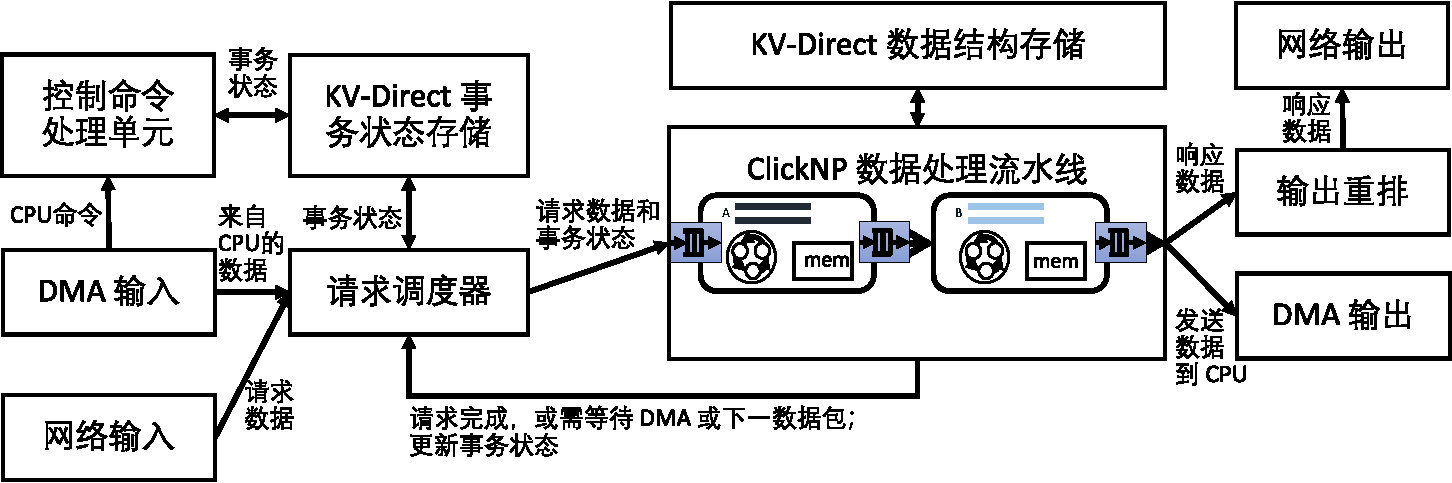
\includegraphics[width=0.6\textwidth]{kvdirect_arch.pdf}
\caption{键值处理器架构。}
\label{kvdirect:fig:kvprocessor-arch}
\end{figure}

如图 \ref {kvdirect:fig:kvprocessor-arch} 所示,键值处理器从板载网卡接收数据包,解码向量操作并将键值操作缓冲在保留站 \footnote{保留站(reservation station)是计算机体系结构中的概念,存储待执行的操作,并调度合适的操作并发执行。} 中(第 \ref {kvdirect:sec:ooo} 节)。
接下来,乱序执行引擎(第 \ref {kvdirect:sec:ooo} 节)从保留站发送可并发执行的键值操作到键值操作译码器。
根据操作类型,键值处理器查找哈希表(第 \ref {kvdirect:sec:hashtable} 节)并执行相应的操作。
为了最小化内存访问次数,较小的键值对在哈希表中内联(inline)存储,其他的键值对存储在 slab 内存分配器(第 \ref {kvdirect:sec:slab} 节)的动态分配内存中。
哈希索引和slab分配的内存都由统一的内存访问引擎(第 \ref {kvdirect:sec:dram-cache} 节)管理,它通过PCIe DMA访问主机内存并将部分主机内存缓存在板载DRAM中。
键值操作完成后,结果被发送回乱序执行引擎(第 \ref {kvdirect:sec:ooo} 节),在保留站中寻找依赖它的键值操作并执行之。

正如第 \ref {kvdirect:sec:challenge} 节所讨论的,PCIe 吞吐量的稀缺性要求键值处理器节约 DMA 访问。
对于 GET 操作,至少需要读取一次内存。
对于 PUT 或 DELETE 操作,对于哈希表数据结构,至少需要一次读取和一次写入 \footnote{读取操作取出哈希槽内的键,如果槽位为空或与待查找的键相同,且不需要重新分配内存空间,则需要一次写入操作来写回数据}。
基于日志的数据结构可以实现每个 PUT 平摊下来少于一次的写入操作,但它牺牲了 GET 性能。
KV-Direct 仔细设计哈希表,以便在每次查找和插入时实现接近理想的 DMA 访问。KV-Direct 也仔细设计了内存分配器,使每次动态内存分配平摊下来,只需不到 0.1 次 DMA 操作。

\subsection{哈希表}
\label{kvdirect:sec:hashtable}

为了存储可变大小的键值,键值存储分为两部分。 第一部分是哈希索引(图 \ref {kvdirect:fig:hashtable}),它包含固定数量的\textit {哈希桶}。 每个哈希桶包含几个\textit {哈希槽}和一些元数据。 内存的其余部分是动态分配的,由slab分配器(第 \ref {kvdirect:sec:slab} 节)管理。
初始化时配置的\textit {哈希索引比率}(hash index ratio)是哈希索引的大小占键值存储总内存大小的比例。
哈希索引比率的选择将在第 \ref {kvdirect:sec:hashtable-eval} 节讨论。


\begin{figure}[htbp]
	\centering
	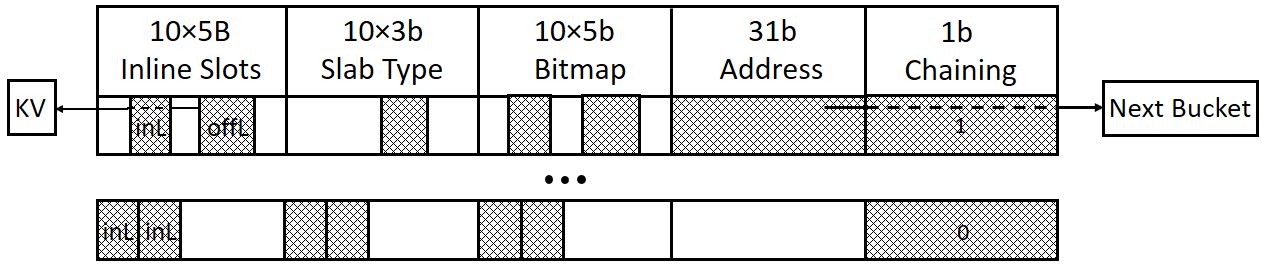
\includegraphics[width=1.0\textwidth,page=1]{hashline.PNG}
	\caption{哈希索引结构。每行是一个哈希桶,包含10个哈希槽,每个哈希槽包括 3 位的 slab 内存类型,一个位图标记内联键值对的开始和结束,以及指向哈希冲突时下一个链接桶的指针。}
	\label{kvdirect:fig:hashtable}
\end{figure}


%\textbf{Hash Table.}
%Each bucket includes 10 hash slots, 3b type code per slot, 50b metadata, plus 31b address and a valid bit of the next chained bucket, as shown in Figure~\ref{kvdirect:fig:hashtable}.
%For offline 键值s, each hash slot needs to store 31b of address, 9b of secondary hash and 3b type code for the slab size.
%For inline 键值s, to mark the begin and end of each hash slot, as well as the separation between inline key and value, the information is encoded in a 50b metadata corresponding to 50 bytes of hash slots.
%The inline keys and secondary hashes of offline keys in all hash slots are compared in parallel, and the first match is found.

每个哈希槽包括指向动态分配的存储器中的键值数据的指针和\textit{辅助哈希}。
辅助哈希是一种优化,采用与主哈希函数独立的另一个哈希函数。由于每个哈希桶中有多个哈希槽,键值处理器需要判断哪个哈希槽对应待查找的键。
通过 9 位的辅助哈希,可以 511/512 的概率确定哪个是待查找的键。但为了确保正确性,仍然需要一次额外的内存访问,将键取出,逐字节比较。
假设主机内存中的64~GiB 键值存储和32字节分配粒度~\footnote{32 字节的分配粒度权衡了内部碎片和用于内存分配的元数据开销。},指针需要31位。
每个哈希槽的大小是 5 字节~\footnote{本文中的设计参数是根据本文所用硬件平台的参数配置的,对于不同容量的内存,哈希槽大小、指针位宽等参数可能改变。}。
为了确定哈希桶大小,需要在每个桶的哈希槽数和 DMA 吞吐量之间进行权衡。
图 \ref {kvdirect:fig:dma-tput} 表明,低于 64B 粒度时,DMA 读取吞吐量受 DMA 引擎中 PCIe 延迟和并行性的约束。
小于 64B 的桶大小将增加哈希冲突的可能性。
另一方面,将桶大小增加到 64B 以上会降低哈希查找的吞吐量。
因此桶大小选择为 64 字节。

\textit {键值大小}是指键和值的总大小。
小于阈值大小的键值在哈希索引中内联(inline)存储,以节约对获取键值数据的额外存储器访问。
内联键值可以跨越多个哈希槽,其指针和辅助哈希字段被重新用于存储键值数据。
内联所有可装入哈希索引的键值可能不是最佳选择。
一个内联的键值可能占用多个哈希槽,减小了哈希表可存储的键值数量。
在哈希表容量允许的情况下,内联键值可以减少平均内存访问次数。
为此,KV-Direct 根据哈希表被填满的比例来选择 \textit {内联阈值},并内联小于该阈值的键值。
传统上,哈希表采用负载因子(load factor) \footnote{负载因子是已被占用的哈希槽数量与总哈希槽数量之比。} 来衡量哈希表被填满的比例,然而这忽略了哈希表的元数据(metadata)和内部碎片(internal fragmentation)带来的开销。为了更科学地比较哈希表不同参数的选择,本章使用 \textit {内存利用率}(memory utilization) \footnote{内存利用率是键值存储中所有键值的大小之和与键值存储的总大小之比。由于元数据和内部碎片的存在,内存利用率总是小于 1 的。}。
如图 \ref {kvdirect:fig:inline-offline} 所示,对于某个内联阈值,由于更多的哈希冲突,每个键值操作的平均内存访问次数随内存利用率的增加而增加。
较高的内联阈值下,平均内存访问次数的增长曲线更陡峭。
因此可以找到最佳内联阈值以最小化在给定内存利用率下的内存访问次数。
与哈希索引比率一样,内联阈值也可以在初始化时配置。


\begin{figure}[htbp]
	\centering
	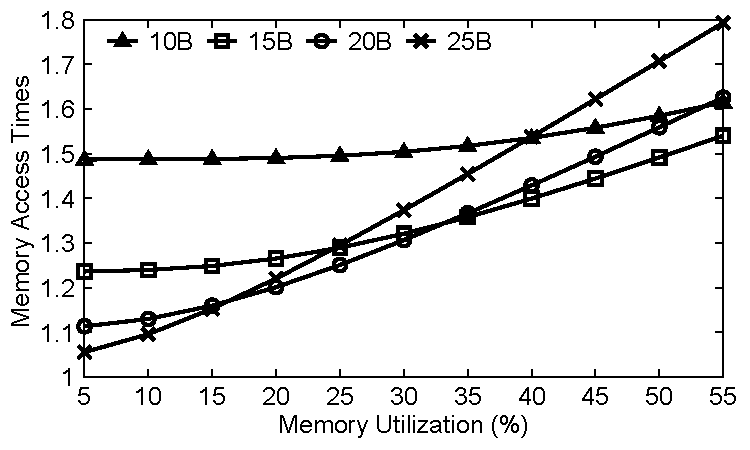
\includegraphics[width=0.6\textwidth]{inline_thresh.pdf}
	\caption{不同内联阈值下的平均内存访问次数和内存利用率。}
	\label{kvdirect:fig:inline-offline}
\end{figure}


当哈希桶中的所有哈希槽都已填满时,有几种解决方案可以解决哈希冲突。
布谷鸟哈希(Cuckoo Hashing)\cite {pagh2004cuckoo} 和跳房子哈希(Hopscotch Hashing)\cite {herlihy2008hopscotch} 通过在插入过程中移动已被占用的哈希槽来保证新插入的键值总是被插入到哈希桶中,从而查找时仅需比较同一哈希桶中恒定数量的哈希槽,实现恒定时间查找。
但是,在写入密集型工作负载中,高负载率下的内存访问时间会有较大的波动。
在极端情况下,甚至可能出现插入失败,需要哈希表扩容的情况。
另一种解决哈希冲突的方法是 \textit{线性探测法},它可能受到群集(clustering)的影响,因此其性能对哈希函数的均匀性敏感。
为此,本文选择 \textit {拉链法} 来解决哈希冲突,这平衡了查找和插入的性能,同时对哈希群集更加健壮。

为了比较 KV-Direct 的拉链法、MemC3中的桶式布谷鸟哈希(bucketized Cuckoo Hash)\cite {fan2013memc3} 和 FaRM \cite {dragojevic2014farm} 中的链式关联(chain associative)跳房子哈希(Hopscotch Hash),图 \ref {kvdirect:fig:mem-access-tput} 绘制了三种可能的哈希表设计中每个GET和PUT操作的平均内存访问次数。
在 KV-Direct 的实验中,针对给定的键值大小和内存利用率要求,为内联阈值和哈希索引比率做出最佳选择。
在布谷鸟和跳房子哈希实验中,假设键是内联的并且可以并行比较,而值存储在动态分配的 slab 存储区中。
由于MemC3和FaRM的哈希表不能对 10B 键值大小支持超过55%的内存利用率(即它们的元数据和内部碎片占用空间较多),图 \ref {kvdirect:fig:mem-access-10-get} 和图 \ref {kvdirect:fig:mem-access-10-put} 仅显示KV-Direct的性能。




\begin{figure}[htbp]
	\centering
	\subfloat[10B GET.\label{kvdirect:fig:mem-access-10-get}]
	{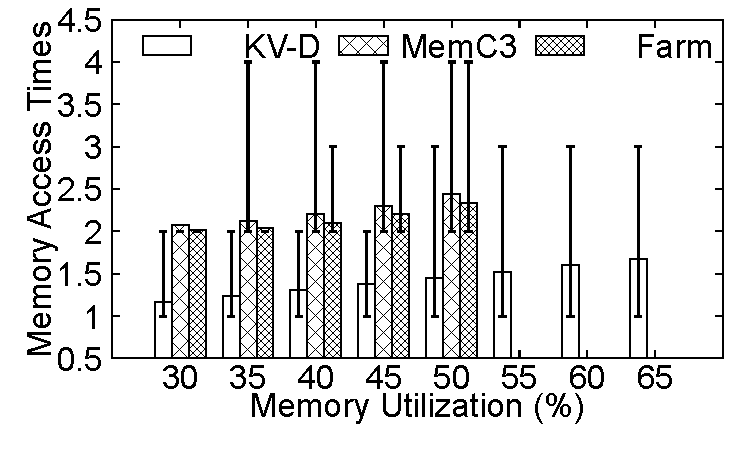
\includegraphics[width=.5\textwidth,page=1]{10B_get.pdf}}
	\subfloat[10B PUT.\label{kvdirect:fig:mem-access-10-put}]
	{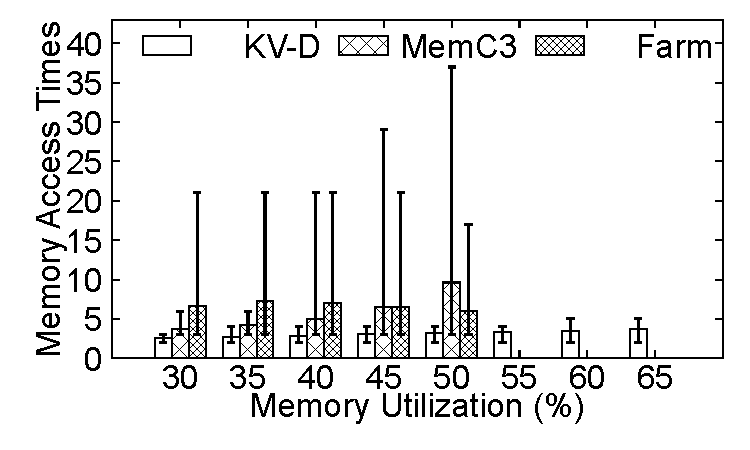
\includegraphics[width=.5\textwidth,page=1]{10B_put.pdf}}
	
	\vfill
	
	\subfloat[254B GET.\label{kvdirect:fig:mem-access-254-get}]
	{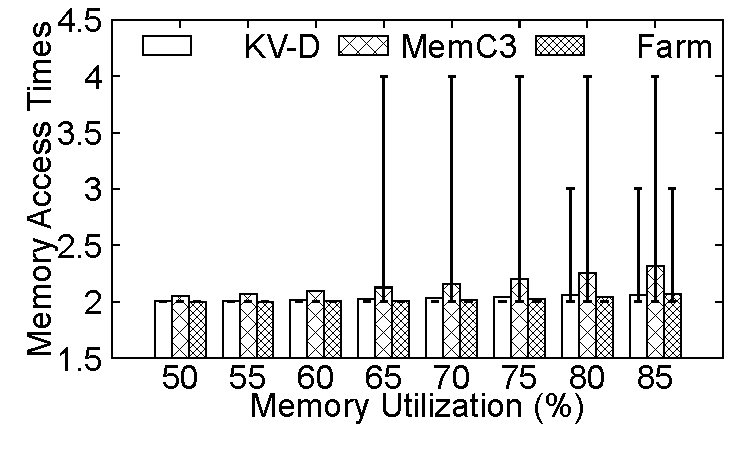
\includegraphics[width=.5\textwidth,page=1]{254B_get.pdf}}
	\subfloat[254B PUT.\label{kvdirect:fig:mem-access-254-put}]
	{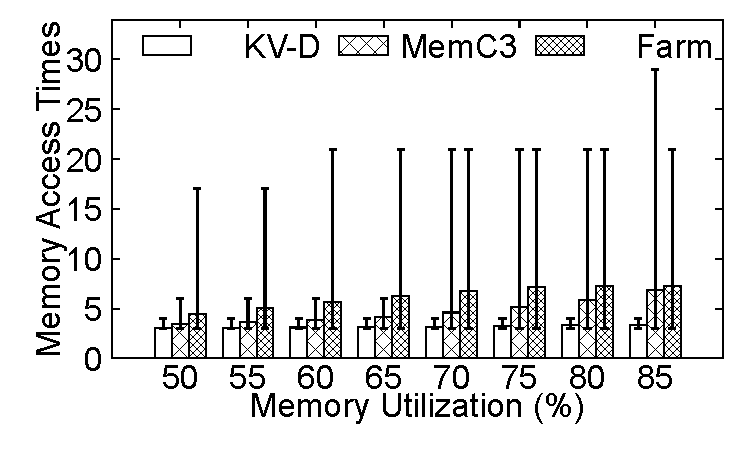
\includegraphics[width=.5\textwidth,page=1]{254B_put.pdf}}
	\caption{每个键值操作的内存访问次数。}
	\label{kvdirect:fig:mem-access-tput}
\end{figure}


对于内联键值,KV-Direct的每个GET操作仅需接近1次内存访问,在非极端内存利用率下每个PUT也仅需2次内存访问。
非内联键值的GET和PUT则有一次额外的内存访问。
在高内存利用率下比较KV-Direct和链式跳房子哈希,跳房子哈希在GET中表现更好,但在PUT中表现更差。
虽然KV-Direct无法保证最坏情况下的DMA访问次数,但会在GET和PUT之间取得平衡。
布谷鸟哈希的GET操作能保证访问最多两个哈希槽,因此在大多数内存利用率下,KV-Direct的内存访问次数更多。
但是,在高内存利用率下,布谷鸟哈希会导致PUT操作的内存访问次数出现大幅波动。


%In KV-Direct, we measure memory utilization instead of load factor, because chaining has dynamic size and that we care more about the overall storage efficiency counting all indexing, metadata and memory fragmentation overhead.
%Clearly, small 键值s cause lower memory utilization due to metadata overhead.
%The optimal hash index ratio is chosen at initialization time according to workload to balance average access time and memory utilization.

\label{kvdirect:sec:hashtable-eval}

哈希表设计中有两个自由参数:(1)内联阈值,(2)整个内存空间中哈希索引的比率。
如图 \ref {kvdirect:fig:optimize_fix_mem} 所示,当哈希索引比率增长时,可以内联存储更多的键值对,从而产生更低的平均内存访问次数。
图 \ref {kvdirect:fig:optimize_fix_ratio} 显示了随着使用更多内存而增加的内存访问次数。


\begin{figure}[htbp]
	\subfloat[固定内存利用率 0.5。\label{kvdirect:fig:optimize_fix_mem}]
	{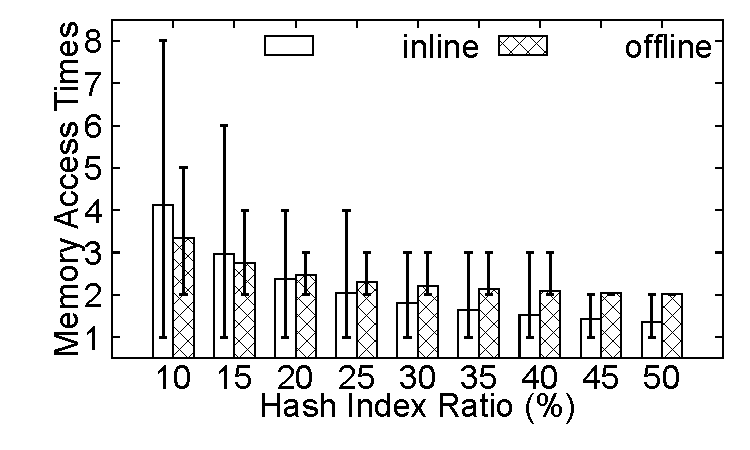
\includegraphics[width=.5\textwidth,page=1]{fix_mem.pdf}}
	\subfloat[固定哈希索引率 0.5。\label{kvdirect:fig:optimize_fix_ratio}]
	{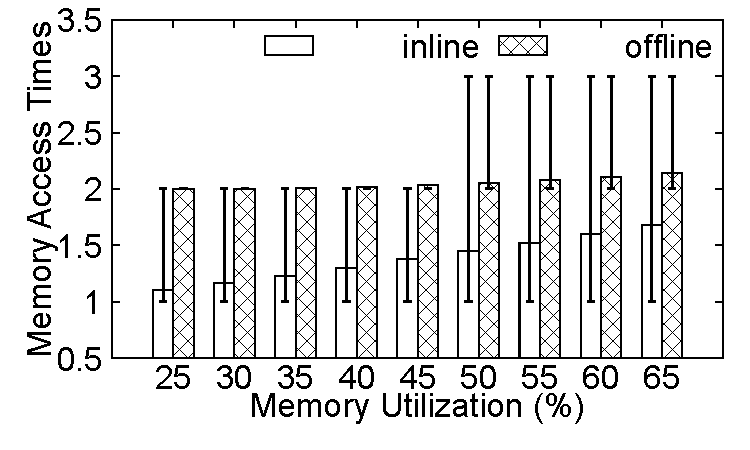
\includegraphics[width=.5\textwidth,page=1]{fix_ratio.pdf}}
	\caption{不同内存利用率或哈希索引率下的内存占用。}
	\label{kvdirect:fig:memory-access-count}
\end{figure}

如图 \ref {kvdirect:fig:hashline-ratio} 所示,最大内存利用率在哈希索引比率较高时下降,因为可用于动态分配的内存较少。
因此,为了在给定的内存空间中容纳所有需存储的键值,哈希索引比率具有上限。
本节选择此上限以获得最小的平均内存访问次数,如图 \ref {kvdirect:fig:hashline-ratio} 中的虚线所示,首先根据目标内存利用率,得到有大的哈希索引比率;然后根据哈希索引比率可以得到理论上 GET 操作查找索引所需的平均内存访问次数。


\begin{figure}[htbp]
	\centering
	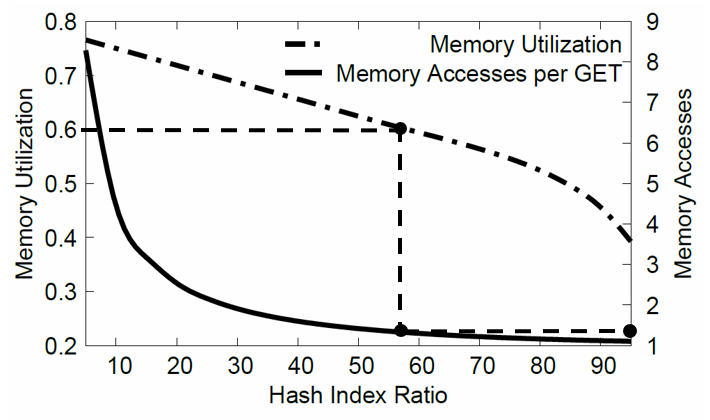
\includegraphics[width=0.6\textwidth,page=1]{optimize.png}
	\caption{如何在给定内存利用率需求和键值大小的情况下决定最优哈希索引率。}
	\label{kvdirect:fig:hashline-ratio}
\end{figure}





\subsection{Slab 内存分配器}
\label{kvdirect:sec:slab}

链式哈希槽和非内联键值需要动态内存分配。
为此,本章选择slab内存分配器 \cite {bonwick1994slab} 来实现每次内存分配和释放的 $O(1)$ 平均内存访问次数。主slab分配器逻辑在主机CPU上运行,并通过PCIe与键值处理器通信。
Slab分配器将分配大小四舍五入到最接近的2的幂,称为\textit {slab 大小}。
它为每个可能的slab大小(32,64,\ldots,512字节)和全局 \textit {分配位图}(allocation bitmap)维护\textit {空闲 slab 池},以帮助将小的空闲slab合并回更大的slab。
每个空闲slab池是一个\textit {slab 条目}数组,由一个地址字段和一个slab类型字段组成。slab类型字段表示slab条目的大小。

可以在网卡上缓存可用的slab池,并与主机内存同步。通过批处理的 PCIe DMA 同步操作,每次分配或释放内存平摊下来只需少于 0.07 次 DMA 操作。
当一个空闲 slab 池几乎是空的时,需要拆分较大的 slab。
因为slab类型已经包含在slab条目中,所以在 \textit {slab 分割} 时,slab条目只需从较大的池复制到较小的池,而不需要分割出多个小 slab 条目。

在重新分配时,slab分配器需要检查释放的slab是否可以与其邻居合并,需要至少一次读取和写入分配位图。
受垃圾收集的启发,主机上的 \textit {懒惰 slab 合并} 在一个slab池几乎为空,并且没有更大的slab池有足够的slab来拆分时,批量合并空闲slab。


\begin{figure}[htbp]
	\centering
	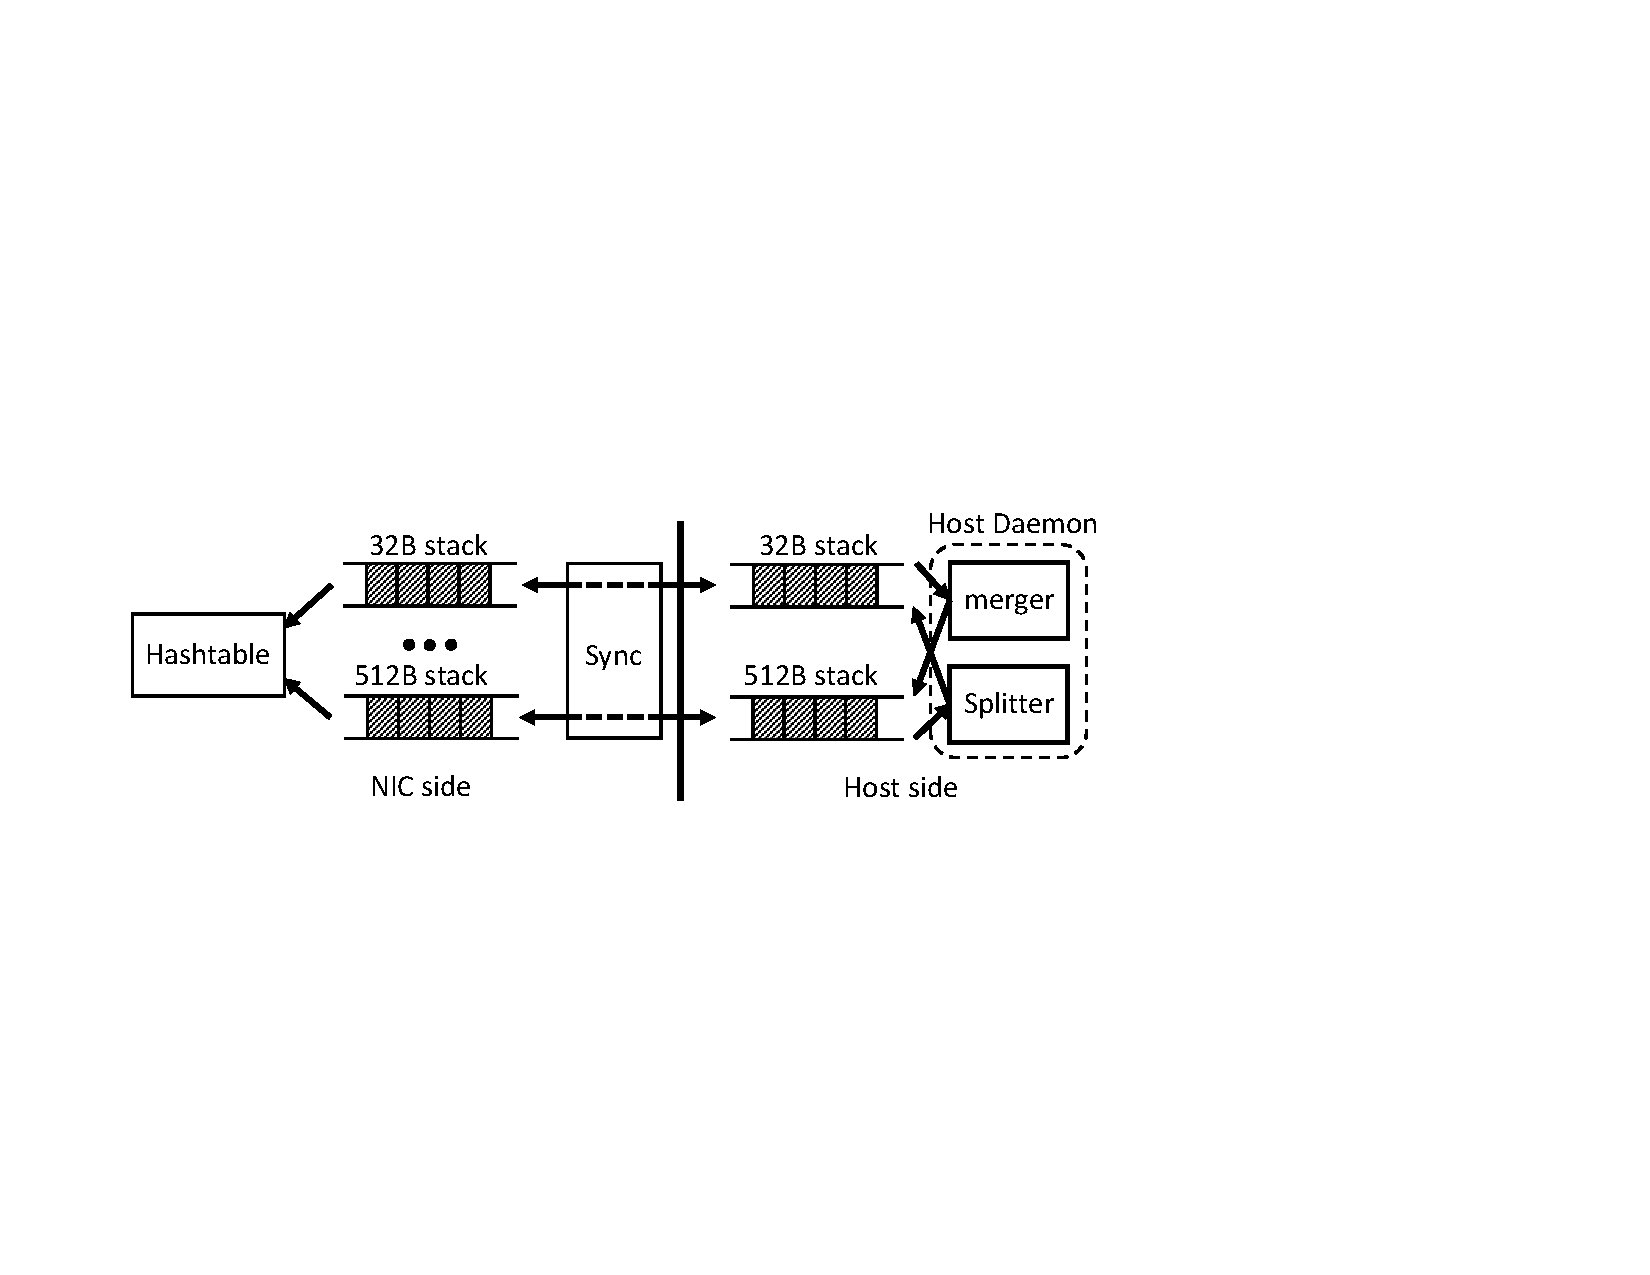
\includegraphics[width=.8\textwidth,page=1]{figure/cropped_slab.pdf}
	\caption{Slab 内存分配器。}
	\label{kvdirect:fig:slab}
\end{figure}

如图 \ref {kvdirect:fig:slab} 所示,对于每个slab大小,网卡上的slab缓存使用两个双端堆栈(double-end stack)与主机DRAM同步。
网卡端的双端堆栈(图 \ref {kvdirect:fig:slab} 中的左侧)左端由分配器出栈、解除分配器入栈,右端通过DMA对应的​​主机端双端堆栈与左端同步。
网卡监视网卡堆栈的大小,并根据高水位线和低水位线与主机堆栈同步。
主机守护进程定期检查主机端双端堆栈的大小。如果高于高水位线,则触发 slab 合并;低于低水位线时,会触发 slab 分裂。
因为双端堆栈的每一端都是仅由网卡或主机之一独占访问的,并且在移动指针之前先搬移数据,所以只要双端堆栈中的数据量大于保护阈值,就不会发生竞争条件。


\label{kvdirect:sec:slab-eval}


Slab内存分配器的通信开销来自网卡访问主机内存中的可用slab队列。
在本章中,每个slab条目是5个字节,DMA粒度是64个字节,因此每个slab操作的平摊DMA开销是$5/64$次DMA操作。此外,网卡上新释放的 slab 槽往往可被网卡后续的分配操作重新使用,因此很多情况下根本不需要 DMA 操作。
为了维持每秒180M操作的最大吞吐量,在最坏的情况下,需要传输180M个slab条目,消耗720 MB/s PCIe吞吐量,即网卡的总PCIe吞吐量的5\%。

Slab内存分配器的计算开销来自主机CPU上的slab拆分和合并。
幸运的是,它们并不经常被调用。
对于具有稳定键值大小分布的工作负载,新释放的slab槽由后续分配重用,因此不会触发拆分和合并。

Slab 拆分需要将连续的slab条目从一个slab队列移动到另一个slab队列。当工作负载从大键值转换到小键值时,在最坏的情况下,CPU需要每秒移动90M个slab 条目,这只占核心的10%,因为它只是连续的内存复制。

将可用slab条目合并到较大的slab条目是相当耗时的任务,因为这个垃圾回收过程需要用 slab 条目的地址填充分配位图,因此需要随机存储器访问。
要对可用slab条目的地址进行排序并合并连续的slab,基数排序 \cite {satish2010fast} 比简单的位图具有更好的多核可扩放性。
如图 \ref {kvdirect:fig:slab-garbage-collection} 所示,将16 GiB向量中的所有40亿个空闲 slab 槽位合并,在一个 CPU 核上需要30秒,而在32个核上使用基数排序仅需1.8秒 \cite{satish2010fast}。
虽然空闲 slab 槽位的垃圾收集需要几秒钟,但它在后台运行而不会停止 slab 分配器,并且实际上仅在工作负载从小键值转换到大键值时触发。


\begin{figure}[t]
	\centering
	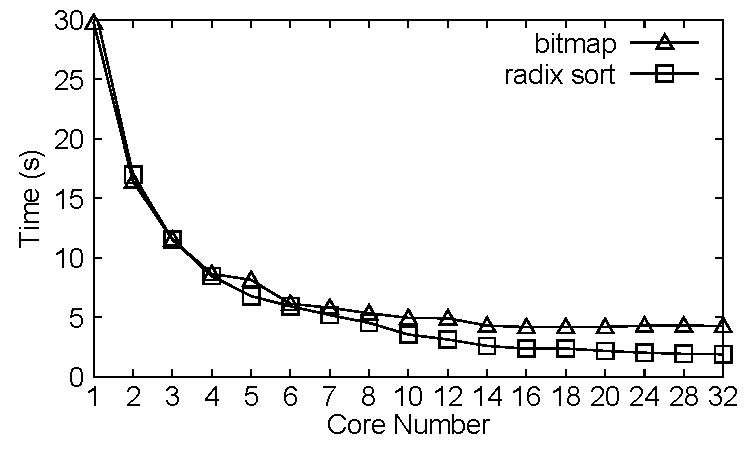
\includegraphics[width=0.6\textwidth]{slab-gc.pdf}
	\caption{合并 40 亿个 slab 槽位的时间开销。}
	\label{kvdirect:fig:slab-garbage-collection}
\end{figure}




\subsection{乱序执行引擎}
\label{kvdirect:sec:ooo}

在键值处理器中,相同键的两个键值操作之间的依赖性将导致数据危险(data hazard)和流水线暂停(pipeline stall)。
在单键原子操作(single-key atomics)中,这个问题更为显著,因为其中所有操作都是有依赖的,必须逐个处理。这限制了原子操作的吞吐量。
本节借用计算机体系结构领域中\textit{动态调度}的概念,并实现 \textit {保留站}(reservation station)来跟踪所有正在进行的键值操作及其 \textit {执行上下文}。

为了饱和利用PCIe、DRAM带宽和处理流水线,需要多达256个并发执行的键值操作。
但是,并行比较256个16字节键将占用FPGA的40\%逻辑资源。
为了避免并行比较,本节将键值操作存储在片上BRAM中的小哈希表中,由键的哈希索引。
相同哈希值的键值操作被视为具有依赖关系。
不同的键可能具有相同的哈希值,因此可能存在误报的依赖关系,但它永远不会错过依赖关系。
具有相同哈希的键值操作组织成链表结构,由键值处理器顺序处理。
哈希冲突会增加误报的依赖关系,降低键值处理效率,因此保留站包含1024个哈希槽,使哈希冲突可能性低于25\%。

保留站不仅保存因依赖关系而暂时挂起的操作,还缓存了最近被访问的键值以便进行 \textit {数据转发}(data forwarding)。
当主处理流水线完成键值操作时,其结果返回给客户端,最新值被转发到保留站。
保留站逐个检查相同哈希槽中的待定操作,立即执行具有匹配键的操作并从保留站移除。
对于原子操作,计算在专用执行引擎中执行。
对于写入操作,将更新缓存的值。
执行结果直接返回给客户端。
在扫描完成依赖关系链表后,如果保留站缓存的值被更新了,则向主处理流水线发出PUT操作,以将高速缓存写回到主存。
这种数据转发和快速执行路径使单键原子操作能够在每个时钟周期内处理一次操作 \footnote{本章中 FPGA 键值处理器的时钟频率是 180 MHz,因此吞吐量可达 180 M op/s。},消除了频繁被访问的键的线头阻塞(head-of-line blocking)。
保留站确保了数据一致性,因为在同一个键上没有两个操作可以在主处理流水线中同时进行。
图 \ref{kvdirect:fig:ooo-mem-access} 描述了乱序执行引擎的结构。

\begin{figure}[htbp]
	\centering
	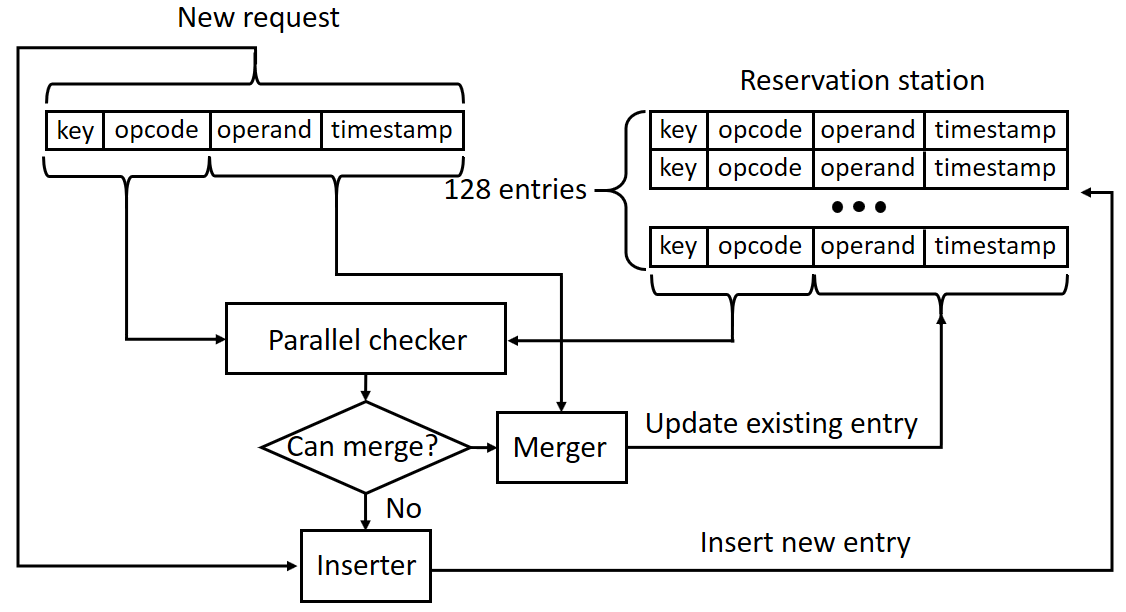
\includegraphics[width=.9\textwidth,page=1]{dynamic_scheduler.PNG}
	\caption{乱序执行引擎。}
	\label{kvdirect:fig:ooo-mem-access}
\end{figure}


\label{kvdirect:sec:ooo-eval}

下面评估乱序执行的有效性。
使用的工作负载包括单键原子操作和长尾分布。
对比方法是遇到键冲突就暂停流水线的简单方法。
使用单边RDMA和双边RDMA \cite {kalia2016design} 吞吐量作为基线。


\begin{figure}[htbp]
	\centering
	\subfloat[原子操作。\label{kvdirect:fig:ooo-atomic}]
	{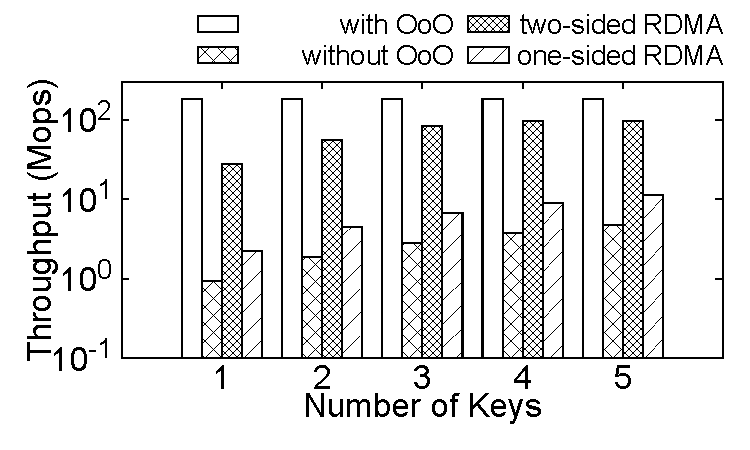
\includegraphics[width=.5\textwidth,page=1]{ooo_atomic.pdf}}
	\subfloat[长尾负载。\label{kvdirect:fig:ooo-longtail}]
	{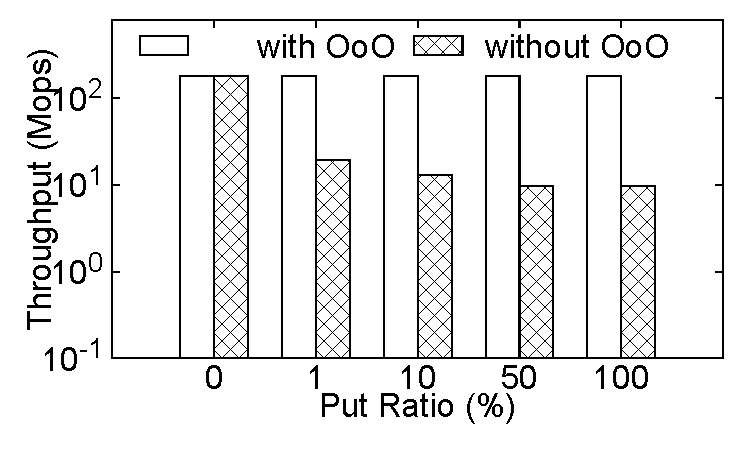
\includegraphics[width=.5\textwidth,page=1]{ooo_long-tail.pdf}}
	\caption{乱序执行引擎的效率。}
	\label{kvdirect:fig:ooo-eval}
\end{figure}

如果没有乱序执行引擎,原子操作需要等待网卡中的PCIe延迟和处理延迟,在此期间无法执行对同一键的后续原子操作。
如图 \ref{kvdirect:fig:ooo-atomic},暂停流水线方法的单键原子操作吞吐量为 0.94~Mops,与使用商用 RDMA 网卡测量的 2.24~Mops 接近 \cite {kalia2016design}。
商用 RDMA 网卡的更高吞吐量可归因于其更高的时钟频率和更低的处理延迟。
利用乱序执行,KV-Direct 的单键原子操作可达峰值吞吐量,即每个时钟周期处理一次键值操作。
在 MICA \cite {lim2014mica} 中,单键原子吞吐量受限于单个 CPU 核的处理能力,无法随多核扩放。
事实上,原子增加(atomic increment)操作的性能可以随多核扩放 \cite {kalia2016design},但它依赖于原子操作之间的可交换性,因此不适用于不可交换的原子操作,如比较-交换(compare and swap)。

利用乱序执行,单键原子吞吐量提高了191倍,达到了180~Mops的时钟频率极限。
当原子操作在多个键之间均匀分布时,单边RDMA、双边RDMA和没有乱序执行的 KV-Direct 吞吐量随着键的数量线性增长,但仍然与 KV-Direct 使用乱序执行后的最佳吞吐量有很大差距。

图 \ref {kvdirect:fig:ooo-longtail} 显示了长尾工作负载下的吞吐量。
当PUT操作发现流水线中有任何正在进行的键相同的操作时,流水线会暂停。
长尾工作负载具有多个访问非常频繁的键,因此具有相同键的两个操作很可能几乎同时到达。
当PUT操作占所有操作的比例更高时,具有相同键的两个操作中更有可能至少一个是PUT操作,从而触发流水线暂停。





\subsection{DRAM 负载分配器}
\label{kvdirect:sec:dram-cache}

为了进一步减轻PCIe的负担,本节在PCIe和网卡板载DRAM之间调度内存访问。
网卡 DRAM具有4~GiB容量和12.8~GB/s的吞吐量,比主机DRAM(64~GiB)上的键值存储存储小一个数量级,并且比PCIe链路(14~GB / s)稍慢。
一种方法是将固定部分的键值存储放入网卡 DRAM中。但是,网卡DRAM太小,只能容纳整个键值存储的一小部分。
另一种方法是使用网卡 DRAM作为主机内存的缓存,但由于网卡 DRAM的吞吐量有限(甚至比 PCIe 的吞吐量更低),吞吐量甚至会降低。


\begin{figure}[htbp]
	\centering
	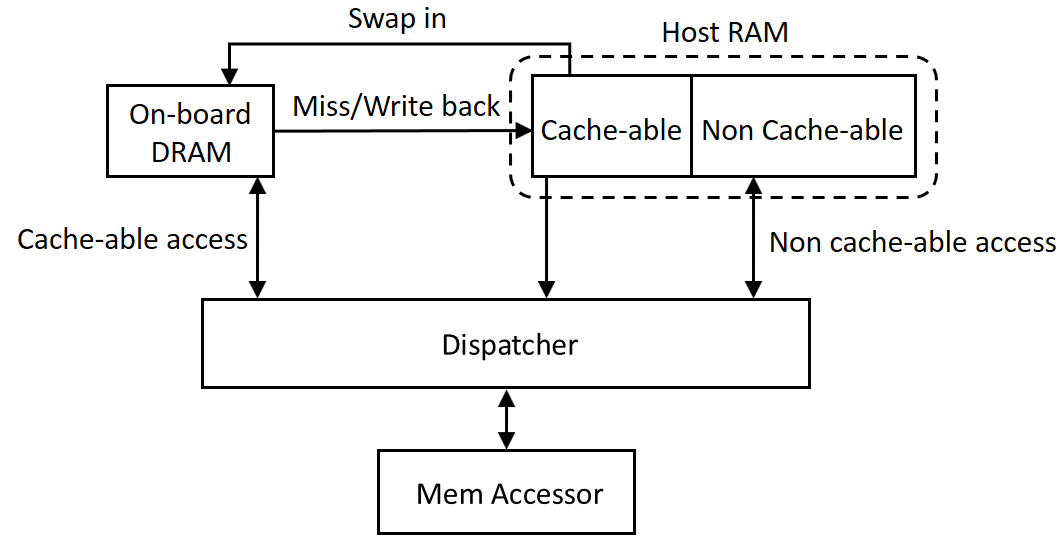
\includegraphics[width=0.8\textwidth,page=1]{load_balancer.PNG}
	\caption{DRAM 负载分配器。}
	\label{kvdirect:fig:cache}
\end{figure}


本节采用混合解决方案,将DRAM用作主机内存中固定部分键值存储的缓存,如图 \ref {kvdirect:fig:cache} 所示。
可缓存部分由存储器地址的哈希确定,哈希的粒度为64字节(DRAM 访存粒度)。
选择哈希函数,使得哈希索引和动态分配的存储器中的地址具有相同的缓存概率。
整个键值存储内存中可缓存内存所占的部分称为\textit {负载分配比例}($ l $)。
如果负载分配比例 $ l $ 增大,更大比例的负载将被分配给板载DRAM,并且缓存命中率 $h(l)$ 将增加。
为了平衡PCIe和板载DRAM上的负载,应优化负载调度比$ l $,使得:
$$\frac{l}{tput_{DRAM}} = \frac{(1-l) + l \cdot (1-h(l))}{tput_{PCIe}}$$

特别的,在均匀(uniform)负载下,令 $k$ 是板上 DRAM 大小和主机键值 存储大小之比,则缓存命中率 $h(l) = \frac{\textnormal{cache size}}{\textnormal{cache-able memory size}} = \frac{k}{l}$。
当 $k \leq l$ 时,均匀负载下的缓存并不高效。
在长尾负载(Zipf 分布)下,设 $n$ 是键值的总数,则大致上 $h(l) = \frac{\log (\textnormal{缓存大小})}{\log (\textnormal{可缓存部分大小})} = \frac{\log (kn)}{\log (ln)}$,当 $k \leq l$ 时。
在长尾工作负载下,1G 的键值存储中 1M 缓存的缓存命中概率高达0.7。
最优的 $l$ 可以得出数值解,这将在第 \ref{kvdirect:sec:different-nic} 节讨论。



一个技术挑战是在DRAM高速缓存中存储元数据。
每64字节的一个缓存行(cache line),需要4个地址位和一个脏标志位的元数据。
因为所有键值存储都由网卡专门访问,不需要缓存有效位。
为了存储每个高速缓存行的5个元数据位,如果将高速缓存行扩展到65个字节,会由于非对齐访问而降低DRAM性能;如果将元数据保存在别处,将使内存访问次数倍增。
相反,本文利用ECC(纠错编码) DRAM中的备用位来进行元数据存储。
ECC DRAM通常每64位数据具有8个ECC位。
事实上,使用汉明码来纠正64位数据中的一位错误,只需要7个额外的校验位。
第8个ECC位是用于检测双位错误的奇偶校验位。
当以64字节粒度和对齐方式访问DRAM时,每64B数据有8个奇偶校验位。
本文将奇偶校验的检查粒度从64个数据位增加到256个数据位,因此仍然可以检测到双位错误。这节约出了6个额外的位,可以用于保存地址位和脏标志这些元数据。


图 \ref {kvdirect:fig:cache-tput} 显示了DRAM负载调度吞吐量相比仅使用PCIe的改进。
在均匀工作负载下,DRAM的缓存效果可以忽略不计,因为它的大小仅为主机键值存储内存的6\%。
在长尾工作负载下,大约30\%的内存访问由DRAM缓存提供。 总的来说,在95\%和100\% GET 情况下,总吞吐量达到了180 Mops的时钟频率限制。
但是,如果简单地将DRAM用作高速缓存,则吞吐量将反而降低,因为DRAM吞吐量低于PCIe吞吐量。


\begin{figure}[htbp]
	\centering
	{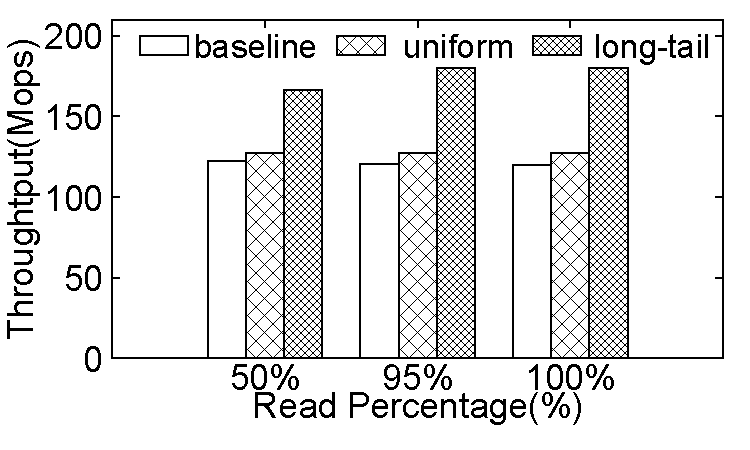
\includegraphics[width=.5\textwidth,page=1]{load_balancer.pdf}}
	\caption{负载分派下的 DMA 吞吐量(固定负载分派比例为 0.5)。}
	\label{kvdirect:fig:cache-tput}
\end{figure}



\subsection{向量操作译码器}

整个键值处理器设计将批处理视为通用原则。
这包括在一个存储桶中批量获取多个哈希槽,空闲slab队列与主机内存的批量同步,懒惰slab拆分和合并,以及保留站对有依赖键值操作沿链表批量处理。
批处理通过将控制平面开销分摊到多个数据平面的有效负载来提高性能。

与PCIe相比,网络是一种更加稀缺的资源,具有更低的带宽(5~GB / s)和更高的延迟(2~$\mu$s)。
以太网上的RDMA写数据包有88字节的包头(header)和填充(padding)开销,而PCIe TLP数据包只有26字节的开销。
这就是以前基于FPGA的键值存储 \cite{blott13hotcloud,blott2015scaling} 没有使PCIe带宽饱和的原因,尽管它们的哈希表设计效率低于KV-Direct。
为了充分利用网络带宽,需要在两个方面进行 \textit {客户端批处理}:在一个数据包中批量处理多个键值操作,并支持向量操作以实现更紧凑的表示。为此,在键值引擎中实现了一个解码器,从单个RDMA数据包中解压缩多个键值操作。
观察到许多键值具有相同的大小或重复值,键值格式包括两个标志位以允许复制键和值大小,或者包中先前键值的值。
幸运的是,许多重要的工作负载(\textit {例如图遍历,参数服务器})的键值操作是可以批量化的。
展望未来,如果可以使用更高带宽的网络,则无需批量处理。


为了评估KV-Direct中向量操作的效率,
表 \ref {kvdirect:tab:vec_throughput} 将原子向量增加(vector increment)的吞吐量与两种替代方法进行比较:
(1)如果每个元素都存储为一个不同的键,则瓶颈是传输键值操作的网络。
(2)如果整个向量存储为一个大的不透明值,由客户端取回处理,则通过网络发送向量的开销也很高。
此外,表 \ref {kvdirect:tab:vec_throughput} 中的两个替代方案不能确保多个客户端同时访问时,向量内部的一致性。 添加客户端间的同步会产生进一步的开销。


\begin{table}[htbp]
	\centering
	\caption{向量操作的吞吐量 (GB/s)。}
	\label{kvdirect:tab:vec_throughput}
	\small
		\begin{tabular}{|l|r|r|r|r|r|}
			\hline
			向量大小 (字节)              & 64    & 128   & 256   & 512   & 1024  \\ \hline
			向量更新(有返回)    & 11.52 & 11.52 & 11.52 & 11.52 & 11.52 \\ \hline
			向量更新(无返回) & 4.37  & 4.53  & 4.62  & 4.66  & 4.68  \\ \hline
			每个元素一个键         & 2.09  & 2.09  & 2.09  & 2.09  & 2.09  \\ \hline
			取回客户端处理             & 0.03  & 0.06  & 0.12  & 0.24  & 0.46  \\ \hline
		\end{tabular}
\end{table}




KV-Direct客户端在网络数据包中打包键值操作,以降低数据包头的开销。
图 \ref {kvdirect:fig:eval-network-batching} 表明,网络批处理可将网络吞吐量提高4倍,同时保持网络延迟低于3.5~$\mu$s。


\begin{figure}[htbp]
	\centering
	\subfloat[吞吐量。\label{kvdirect:fig:network-batching-bw}]
	{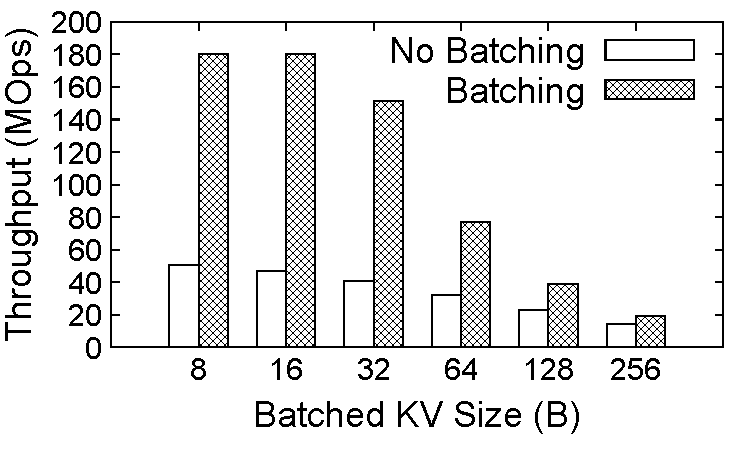
\includegraphics[width=.5\textwidth,page=1]{net_batching_bw.pdf}}
	\subfloat[延迟。\label{kvdirect:fig:network-batching-lat}]
	{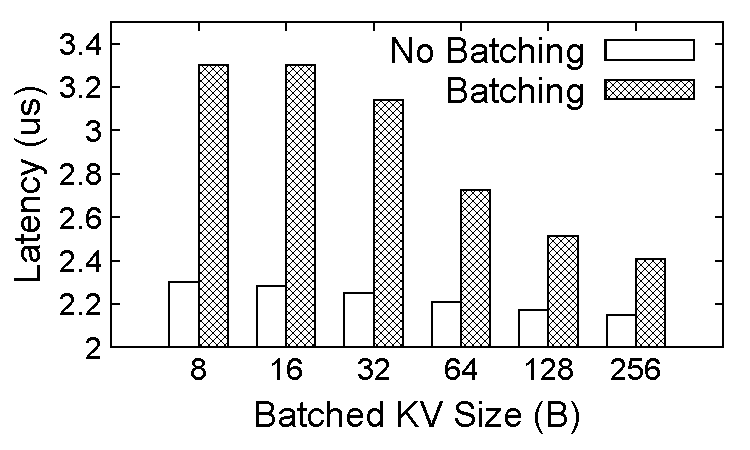
\includegraphics[width=.5\textwidth,page=1]{net_batching_lat.pdf}}
	\caption{网络批量化的效率。}
	\label{kvdirect:fig:eval-network-batching}
\end{figure}

\egg{
\subsubsection{Congestion Avoidance}
\label{kvdirect:sec:congestion-avoidance}

In addition to throughput, another important factor is latency.
From the client's perspective, the 键值 processor is a path with multiple bottlenecks and buffers, \eg, PCIe and DRAM access.
If all buffers in the 键值 processor are filled up, the GET latency would exceed 10~$\mu$s.
To mitigate the bufferbloat problem, we implement a congestion avoidance logic to limit the number of in-flight 键值 operations \textit{inside the 键值 processor}.
The 键值 processor maintains a \textit{键值 operation window} and leverages credit-based flow control mechanism in RDMA to back-pressure 键值存储 clients.
To adapt 键值 operation window size to the workload, we measure the running average of 键值 processing delay and adjust the window size according to TCP Vegas congestion avoidance algorithm~\cite{brakmo1995tcp}.
%We use delay as the congestion signal instead of ECN, because the queues whose sizes are hard to measure.
}
